\documentclass{beamer}
\usetheme{Madrid}
\usecolortheme{spruce}

% Number captions
\setbeamertemplate{caption}[numbered]

% Number bibliography entries
\setbeamertemplate{bibliography item}{\insertbiblabel}

% Change base colour beamer@blendedblue (originally RGB: 0.2,0.2,0.7)
\colorlet{beamer@blendedblue}{green!40!black}

\usepackage{lmodern}
\usepackage{caption}

\usepackage[citestyle=authoryear, sorting=none]{biblatex}
\addbibresource{databall.bib}
\DeclareNameAlias{sortname}{last-first}
\DeclareNameAlias{default}{last-first}

\title{DataBall}
\subtitle{Betting on the NBA with Data}
\author{Kevin Lane}

\begin{document}

\begin{frame}
\titlepage
\end{frame}

\begin{frame}
\frametitle{Outline}
\tableofcontents
\end{frame}

\section{Introduction}

\subsection{Background}
\begin{frame}
\frametitle{Background}
\begin{itemize}
    \item Sports analytics began in professional baseball, most notably with the work of Bill James\footcite{james}
    \begin{itemize}
        \item James coined the term sabermetrics as ``the search for objective knowledge about baseball''
        \item James selected the name to honor the Society for American Baseball Research (SABR)
    \end{itemize}
    \item Gained widespread adoption after Billy Beane implemented James' ideas and led the Oakland Athletics to a record winning streak\footcite{lewis}
    \item Analytics has since spread to other sports and its impact is evidenced by several examples:
    \begin{itemize}
        \item MLB's increased attention to on-base percentage beginning in the Moneyball era of the early 2000s
        \item The rise of the three-point shot and subsequent fall of the midrange jumper in the NBA
        \item Increased use of short, high percentage passes in the NFL
    \end{itemize}
\end{itemize}
\end{frame}

\begin{frame}
\frametitle{Background}
\begin{block}{What makes sports an attractive testbed for machine learning?}
According to Nate Silver, ``sports nerds have it easy.''\footnotemark
\begin{enumerate}
    \item ``Sports has awesome data.''
    \item ``In sports, we know the rules.''
    \item ``Sports offers fast feedback and clear marks of success.''
\end{enumerate}
\end{block}
\footcitetext{silver-online}
\vspace{-0.5cm}
\begin{block}{Why the NBA?}
\begin{itemize}
    \item Easily the most deterministic of the major American sports
    \item The NBA provides a wealth of advanced stats and player tracking data on their website
    \item The season is long enough at 82 games that sample size is not as much of a concern as in the NFL, who claim to have parity, but also only play 16 regular season games
\end{itemize}
\end{block}
\end{frame}

\subsection{Process}
\begin{frame}
\frametitle{Process}
\begin{itemize}
    \item I used several algorithms from the popular Python machine learning library scikit-learn\footcite{scikit-learn} to predict NBA game winners against the spread
    \begin{itemize}
        \item Logistic Regression
        \item Support Vector Machine
        \item Random Forest
        \item Multilayer Perceptron
    \end{itemize}
    \item I collected box scores, point spreads, and over/under lines from the 1990-91 season through 2016-17
    \item I used the 2016-17 season as my test set and trained models with prior seasons
    \item All models are trained with stats averaged over a rolling window
    \begin{itemize}
        \item The stats were shifted so that stats were not used to predict the game from which they were obtained
        \item This provides a realistic scenario for making predictions in real time, such as in betting
    \end{itemize}
\end{itemize}
\end{frame}

\section{Data}

\subsection{Data Wrangling}
\begin{frame}
\frametitle{Data Wrangling}
\begin{itemize}
    \item I collected stats from the NBA's stats website \url{stats.nba.com}
    \begin{itemize}
        \item The site exposes a wealth of information in JSON format through various web API endpoints
        \item I utilized the Python module nba\_py to format URLs and collect stats
    \end{itemize}
    \item I scraped point spreads and over/under lines from covers.com using the Python web scraping framework Scrapy
    \item I stored all data to a SQLite database using Python's built-in support
    \item I used the basic box score stats to calculate more advanced stats
    \begin{itemize}
        \item Offensive/defensive ratings (points scored/allowed per 100 possessions), which requires an estimate for the number of possessions
        \item Simple Rating System (SRS), which is a team's average margin of victory adjusted for its strength of schedule
        \item Oliver's four factors\footcite{oliver}, which include effective FG\%, TOV\%, OREB\%, and free throw rate
        \item Weighted four factors, which is just sum of the four factors weighted according to Oliver's assigned weights
    \end{itemize}
\end{itemize}
\end{frame}

\subsection{Data Exploration}
\begin{frame}
\frametitle{Data Exploration}
\begin{columns}
\column{0.5\textwidth}
\begin{itemize}
    \item The top figure shows that the home team winning percentage is remarkably consistent
    \item Teams only win about half the time against the spread (ATS)
    \begin{itemize}
        \item This provides a tougher problem than picking game winners straight up
    \end{itemize}
    \item The bottom figure shows that home point spreads favor the home teams
    \begin{itemize}
        \item The betting lines indicate home court advantage is about 3.4 points
        \item The distribution is bimodal because oddsmakers rarely set a spread of zero
    \end{itemize}
\end{itemize}
\column{0.5\textwidth}
\vspace{-0.5cm}
\begin{figure}
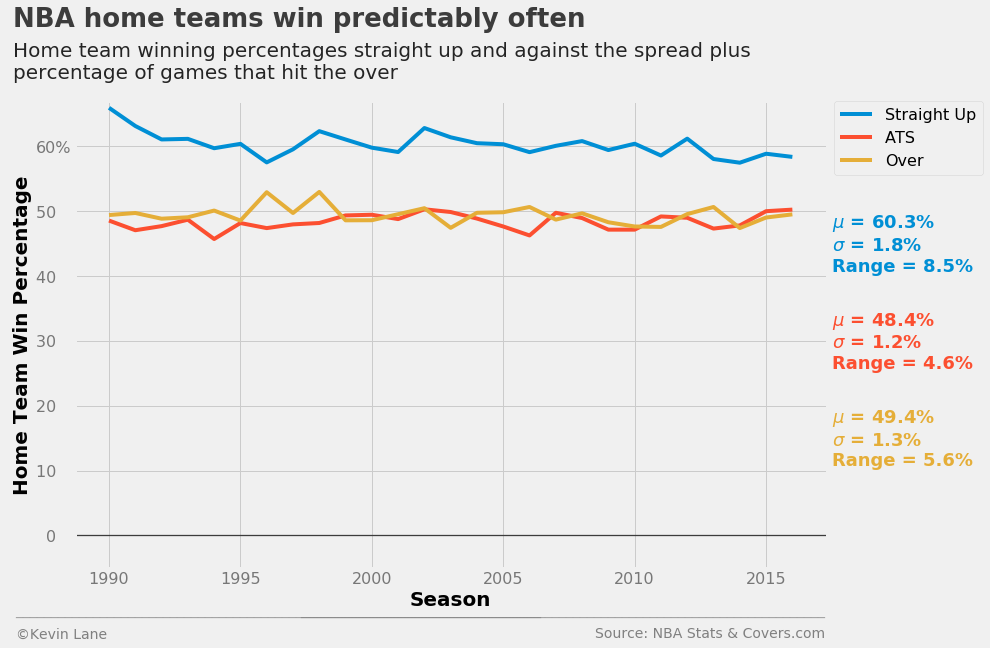
\includegraphics[width=60mm]{../docs/assets/images/data-exploration/home-win-pct.png}
\end{figure}
\vspace{-0.5cm}
\begin{figure}
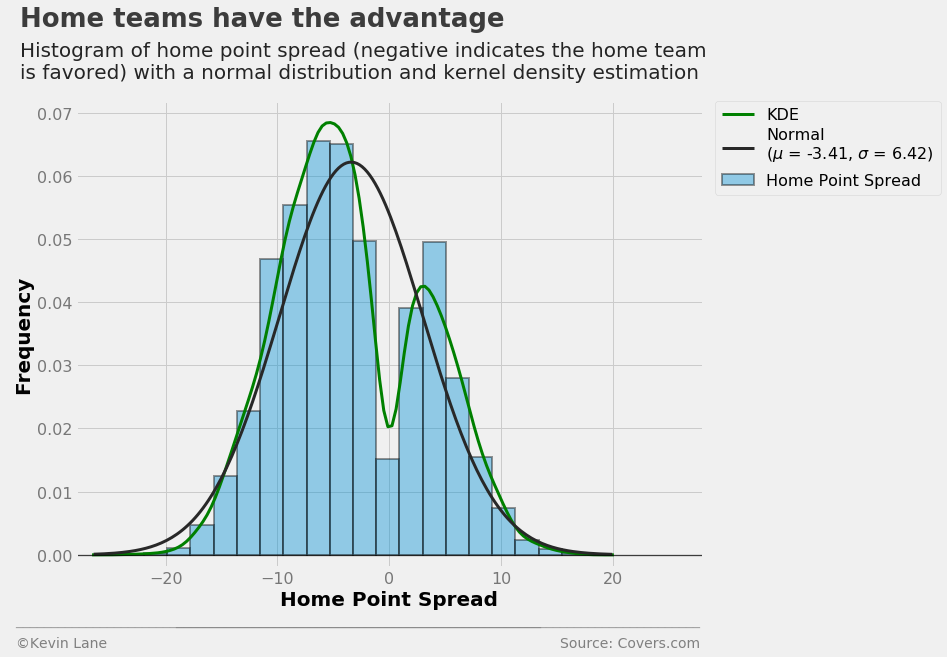
\includegraphics[width=60mm]{../docs/assets/images/data-exploration/point-spread-distribution.png}
\end{figure}
\end{columns}
\end{frame}

\begin{frame}
\frametitle{Data Exploration}
\begin{itemize}
    \item The plots below show kernel density estimations (KDE) of net rating split between home team wins and losses
    \item The dark region to the bottom right of the origin for home team wins shows above-average home teams tend to beat below-average visitors
    \item The opposite appears in the KDE of home team losses
\end{itemize}
\begin{figure}
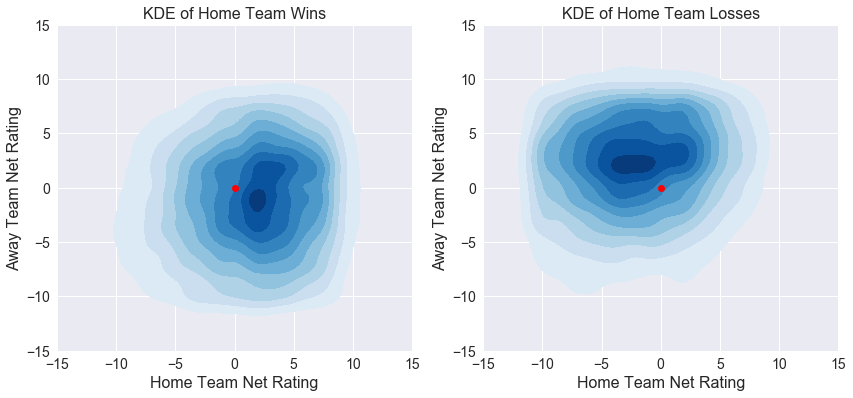
\includegraphics[scale=0.35]{../docs/assets/images/data-exploration/net-rating-win-loss-kde.png}
\end{figure}
\end{frame}

\begin{frame}
\frametitle{Data Exploration}
\begin{columns}
\column{0.5\textwidth}
\begin{itemize}
    \item The plot to the right shows a kernel density estimation (KDE) comparing home point spread with the difference in net rating between the two teams playing in the game
    \item The highest density of points occurs at a positive net rating difference and a negative point spread
    \begin{itemize}
        \item A positive net rating difference indicates the home team is stronger
        \item A negative point spread means the home team is favored
    \end{itemize}
\end{itemize}
\column{0.5\textwidth}
\begin{figure}
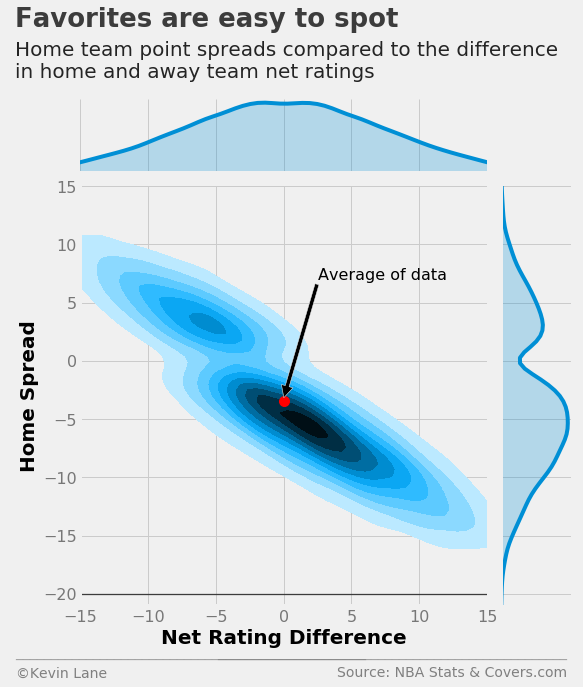
\includegraphics[scale=0.25]{../docs/assets/images/data-exploration/point-spread-kde.png}
\end{figure}
\end{columns}
\end{frame}

\section{Model Selection}

\subsection{Feature Selection}
\begin{frame}
\frametitle{Feature Selection}
\begin{itemize}
    \item Picking winners ATS is much harder than picking winners straight up
    \item Simply picking the favorite wins ATS will only be right half the time
\end{itemize}
\begin{figure}
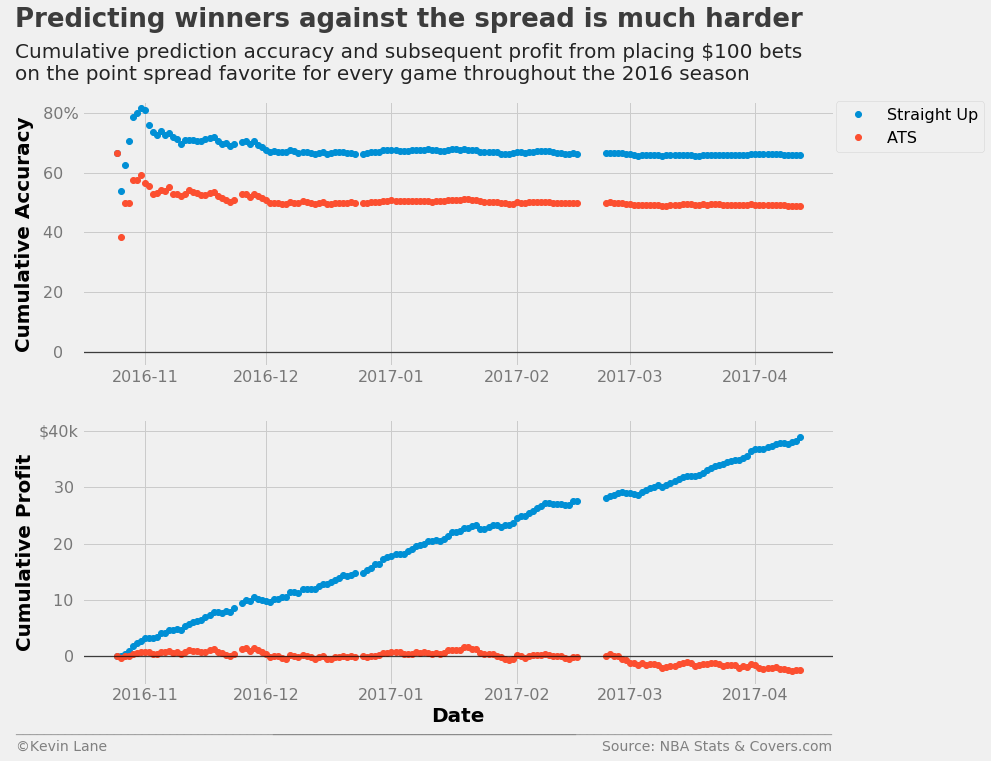
\includegraphics[scale=0.2]{../docs/assets/images/feature-selection/favorite-ats-profit.png}
\caption{Comparison of Betting on Games Straight Up and ATS}
\end{figure}
\end{frame}

\begin{frame}
\frametitle{Feature Selection}
\begin{itemize}
    \item The plots below show cross-validation ROC and precision/recall curves for various metrics
    \item None of the models perform particularly well
\end{itemize}
\begin{figure}
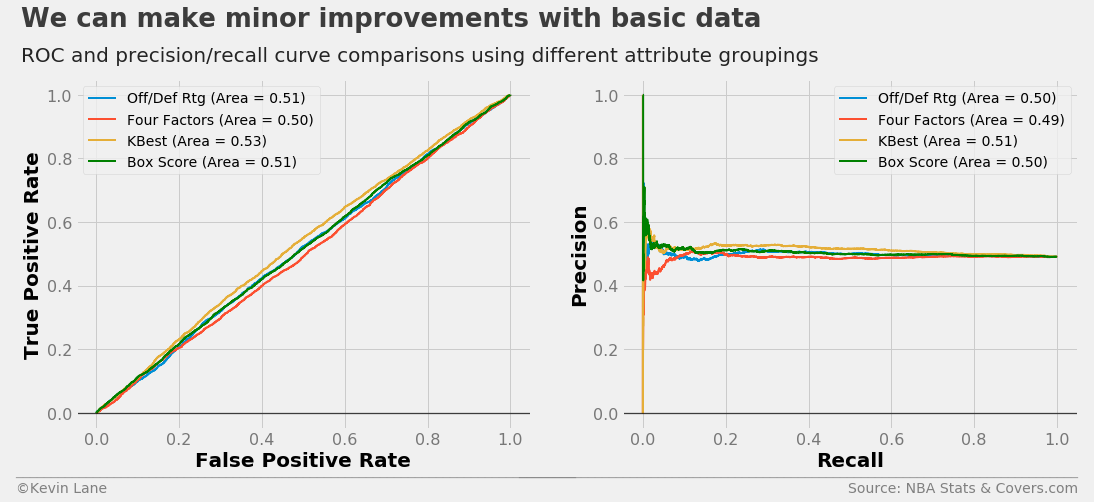
\includegraphics[scale=0.25]{../docs/assets/images/feature-selection/cross-validation-comparison.png}
\caption{ROC and Precision/Recall Curve Feature Comparison}
\end{figure}
\end{frame}

\subsection{Parameter Tuning}
\begin{frame}
\frametitle{Parameter Tuning}
\begin{itemize}
    \item I used the Python module hyperopt to optimize model parameters
    \item It provides a flexible framework for optimizing any scikit-learn classifier
\end{itemize}
\begin{figure}
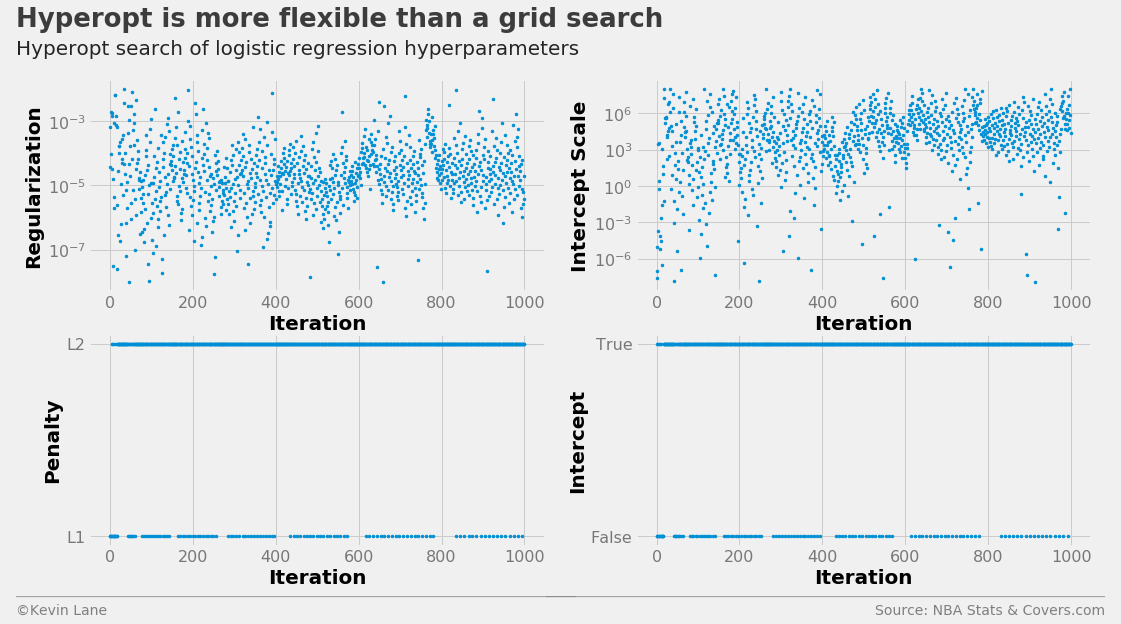
\includegraphics[scale=0.25]{../docs/assets/images/parameter-tuning/logistic-regression-hyperopt.png}
\caption{Logistic Regression Hyperopt Parameter Tuning}
\end{figure}
\end{frame}

\begin{frame}
\frametitle{Parameter Tuning}
\begin{itemize}
    \item Parameter tuning yielded marginal benefits for logistic regression
    \item None of the optimized models performed substantially better than models with default parameters
\end{itemize}
\begin{figure}
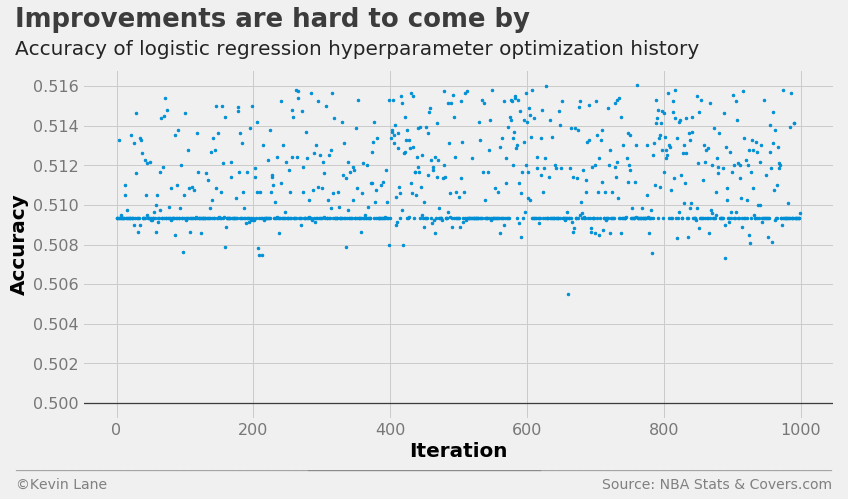
\includegraphics[scale=0.3]{../docs/assets/images/parameter-tuning/logistic-regression-accuracy.png}
\caption{Logistic Regression Accuracy History}
\end{figure}
\end{frame}

\section{Results \& Future Work}

\subsection{Model Performance}
\begin{frame}
\frametitle{Model Performance}
\begin{columns}
\column{0.5\textwidth}
\begin{itemize}
    \item Logistic regression does a decent job at predicting home wins, but struggles with home losses
    \begin{itemize}
        \item The confusion matrix shows the model tends to predict the home team wins
    \end{itemize}
    \item None of the models performed particularly well
    \begin{itemize}
        \item The maximum accuracy was below 55\%
    \end{itemize}
    \item Any accuracy above 50\% will result in a profit
    \begin{itemize}
        \item A 1\% improvement over the course of a season results in about \$2,500 extra when betting \$100 on every game
    \end{itemize}
\end{itemize}
\column{0.5\textwidth}
\begin{figure}
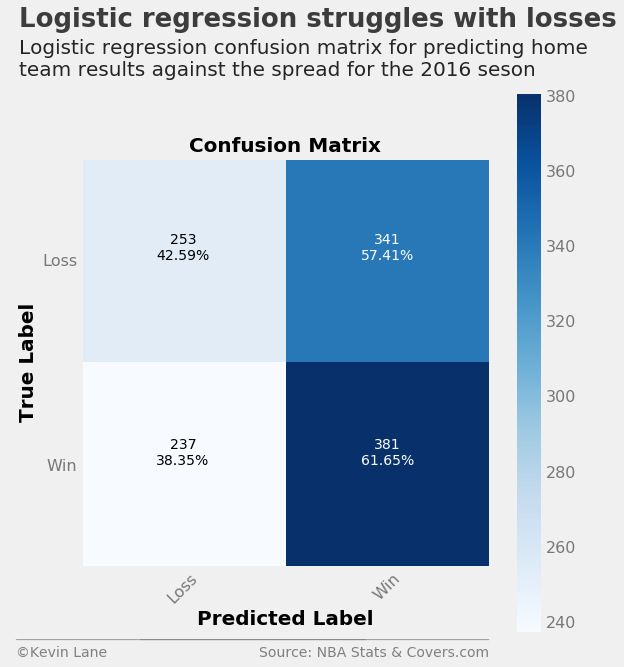
\includegraphics[scale=0.25]{../docs/assets/images/model-performance/logistic-regression-confusion-matrix.png}
\caption{\tabular[t]{@{}l@{}}Logistic Regression \\ Confusion Matrix\endtabular}
\end{figure}
\end{columns}
\end{frame}

\begin{frame}
\frametitle{Model Performance}
\begin{itemize}
    \item The neural network was the highest earning model
    \item All models with optimized parameters returned a profit
\end{itemize}
\begin{figure}
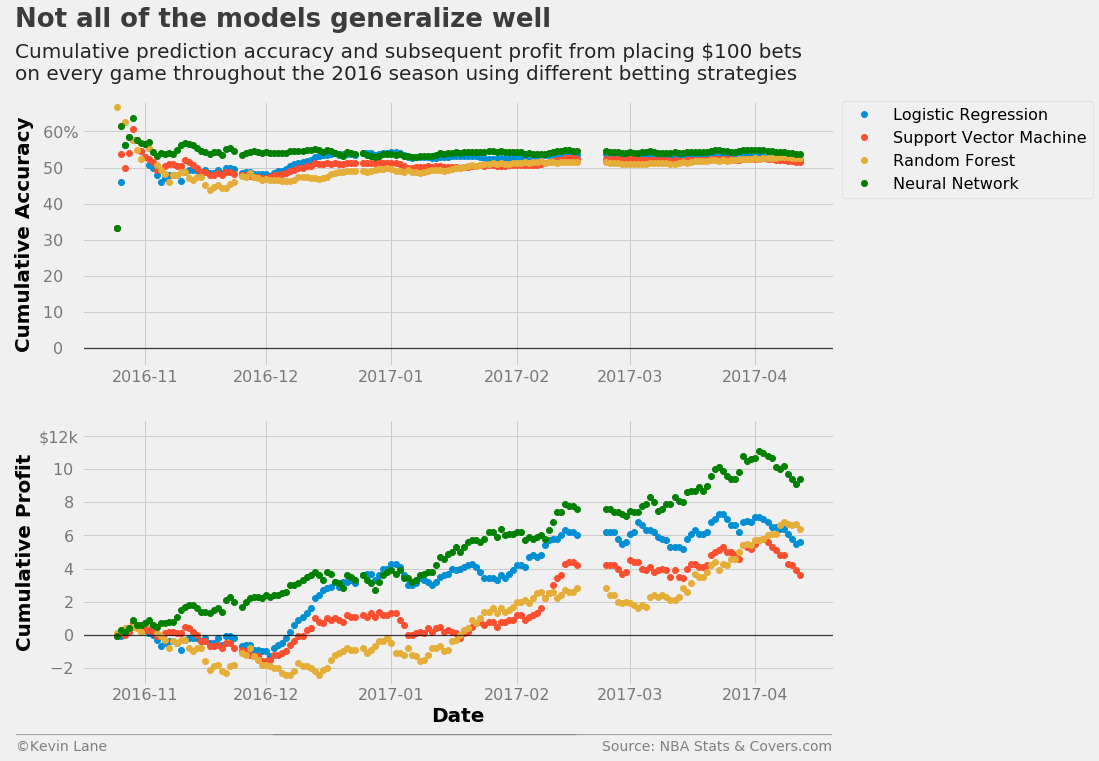
\includegraphics[scale=0.2]{../docs/assets/images/model-performance/model-performance-comparison.png}
\caption{Model Performance Comparison}
\end{figure}
\end{frame}

\begin{frame}
\frametitle{Model Performance}
\begin{itemize}
    \item The hyperparameters optimized prior to the 2016 season did not work well for the logistic regression model
    \item Logistic regression with default parameters earned almost double
\end{itemize}
\begin{figure}
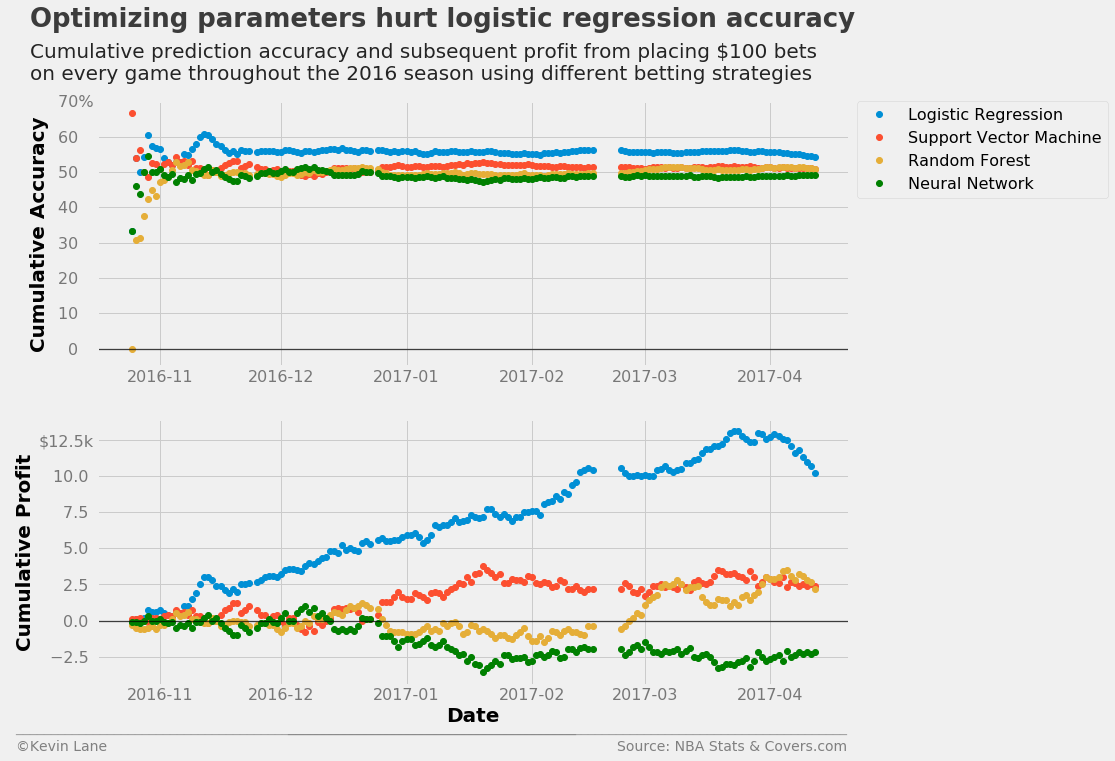
\includegraphics[scale=0.2]{../docs/assets/images/model-performance/default-model-performance-comparison.png}
\caption{Default Model Performance Comparison}
\end{figure}
\end{frame}

\subsection{Future Work}
\begin{frame}[t]
\frametitle{Future Work}
\begin{itemize}
    \item Incorporate player stats to adjust predictions as rosters fluctuate and players sit for rest or injury
    \item Test how well models generalize by predicting other seasons
    \item Calculate stats relative to league average to control for opponent strength and league-wide changes in game strategy
    \item Include a dummy variable indicating if teams are playing the second game of a back-to-back
    \item Predict games against over/under lines
\end{itemize}
\end{frame}

\section{References}

\begin{frame}[t]
\frametitle{References}
\printbibliography
\end{frame}

\end{document}
